\chapter{Self-testing via KS non-contextuality inequalities}
\lhead{\emph{Self-testing via KS non-contextuality inequalities}}
\label{sec:contselftesting}

\section{Preceding results and improvements}

In Section \ref{sec:csw}, we considered general correlation experiments testing some linear combination of probabilities $S$ and found that any quantum realization $\ket{\Psi}$, $\Pi_i$ can be translated into a feasible solution $X$ of the Lovász SDP \ref{eqn:lovaszsdp}, such that the value of $S$, as predicted by QM, corresponds to the objective function the SDP aims to maximize, evaluated at the feasible solution $X$. Conversely, if there are no additional physical constraints, for example due to space-like separated subsystems, one can construct a quantum realization for every feasible solution $X$ that achieves $S=\sum_{i=1}^n X_{ii}$. Such quantum realization was constructed from an arbitrary Gram decomposition of $X$. This connection between feasible solutions to the Lovász SDP and quantum models of the correlation experiment will be central to proving robust self-testing based on KS non-contextuality inequalities.

As outlined in Section \ref{sec:self-testing}, the essence of self-testing is that a maximal violation of suitable Bell or KS non-contextuality inequalities is only compatible with an essentially unique quantum realization $\ket{\Psi}$, $\{\Pi_i\}_i$, up to statistics-preserving trivial degrees of freedom. Furthermore, the inequalities are tests of non-classicality. If our experiment produces correlations that violate these, this certifies that the correlations were not simulated by some classical mechanism, which would render all proofs of information-theoretic security superfluous. Extra care has to be taken in the case of contextuality scenarios, as will be the topic of Section \ref{sec:memoryass}. Ideally, such self-tests should be robust to noise, i.e.\ a $\epsilon$-suboptimal violation should imply that the only compatible quantum realizations are ``close" to the ideal reference implementation, up to trivial degrees of freedom.

We will now sketch the proof in \cite{Bharti2019}, which demonstrates that the class of odd $n$-cycle contextuality scenarios allows for robust self-testing. Recall that an odd $n$-cycle correlation experiment assumes cyclic compatibility relations, like in Figure \ref{fig:kcbscompat}. The self-testing protocol consists of an experimenter choosing freely between the $n$ measurement contexts $(i,i\oplus1)$ and determining the outcome correlations $p(0,1\thinspace\vert\thinspace i,i\oplus 1)$ that constitute the test $S$. The main ``ingredients" of the proof are the following three lemmas:

\begin{lemma}[\cite{Bharti2019}]
\label{lem:kcbsunique}
For the class of odd $n$-cycle exclusivity graphs, $n\geq5$, the Lovász SDP \ref{eqn:lovaszsdp} has a unique optimal solution $X^*_n$.   
\end{lemma}

From Section \ref{sec:cswhierarch} we know that the reference quantum experiment $\{\vert u_j^{(n)} \rangle \}_{j=0}^{n}$ presented in Section \ref{sec:kcbs} produces a maximal violation of the odd $n$-cycle KS non-contextuality inequality, because it attains the Lovász bound. The unique optimal solution $X^*_n$ is obtained from this reference quantum realization by the usual procedure:
\begin{equation*}
    X^*_n=\operatorname{Gram}(\thinspace\vert u_0 \rangle\thinspace,\thinspace \langle u_1^{(n)} \vert u_0 \rangle \vert u_1^{(n)} \rangle\thinspace,\thinspace\dots,\thinspace \langle u_n^{(n)} \vert u_0 \rangle \vert u_n^{(n)} \rangle\thinspace)\thinspace.
\end{equation*}

The following two lemmas will be important to prove robustness:

\begin{lemma}[\cite{Bharti2019}]
\label{lem:epssuboptgram}
Let $(\mathcal{G}_{ex},w)$ be a weighted exclusivity graph with $n$ vertices and assume that \ref{eqn:lovaszsdp} has a unique optimal solution $X^*\in \mathcal{S}_+^{\thinspace n+1}$. Further, let $\Tilde{X}$ be a feasible solution of \ref{eqn:lovaszsdp} that is $\epsilon$-suboptimal, i.e.\
\begin{equation*}
    \sum_{i=1}^n w_i\thinspace\Tilde{X}_{ii} \geq B_{q}(\mathcal{G}_{ex},w)-\epsilon,
\end{equation*}
where $B_{q}(\mathcal{G}_{ex},w)=\sum_{i=1}^n w_i X_{ii}^*$ is the optimal value of the Lovász SDP for the weighted exclusivity graph $(\mathcal{G}_{ex},w)$.
Then
\begin{equation*}
\|\Tilde{X}-X^*\|_F \leq \mathcal{O}(\epsilon)\,,
\end{equation*}
where $\|A\|_F=\operatorname{tr}(A^{\dag}A)$ is the Frobenius norm.
\end{lemma}

\begin{lemma}
\label{lem:closegramdecomp}
Let $\Tilde{X}\in S_{+}^{\thinspace n+1}$ be a positive semi-definite matrix, $\epsilon$-close to $X^*\in S_{+}^{\thinspace n+1}$ like in \ref{lem:kcbsunique}
\begin{equation*}
\|\Tilde{X}-X^*\|_F \leq \epsilon.
\end{equation*}
Let $\{\vert \Tilde{u}_i \rangle\}_{i=0}^n\subset\mathbb{C}^{d}$ and $\{\vert u_i\rangle\}_{i=0}^n\subset\mathbb{C}^{d}$ be Gram decompositions of $\Tilde{X}$ and $X^*$, respectively. Then there exists a $d\times d$ unitary matrix $U$ such that for all $i\in\{0,\dots,n\}$
\begin{equation*}
    \|\vert \Tilde{u}_i\rangle - U \vert u_i\rangle\|_2 \leq \kappa(n)\epsilon + \mathcal{O}(\kappa(n)^2\epsilon^2)\,,
\end{equation*}
where $\kappa(n)=1+\frac{1}{2}\sqrt{n+4}$ for all $n>7$.
\end{lemma}

We will omit the proofs of Lemmas \ref{lem:kcbsunique} and \ref{lem:epssuboptgram}, as they do not provide much conceptual insight, and offer only a few comments. We include the proof of Lemma \ref{lem:closegramdecomp}, as \cite{Bharti2019} proves only a weaker version, in the sense that $d=n$. More importantly, the proof we present establishes a tighter error bound of the order $\mathcal{O}(\kappa(n)\epsilon)$, compared to $\mathcal{O}(\sqrt{(n+1)\epsilon}\,)$ in \cite{Bharti2019}. As opposed to the result in \cite{Bharti2019}, the proof of Lemma \ref{lem:closegramdecomp} makes use of the fact that the verifier has knowledge about the ideal Gram matrix $X^*$. 

The proof of Lemma \ref{lem:kcbsunique} utilizes SDP duality theory and shows a sufficient condition for the unicity of $X^*_n$ to be satisfied by explicit construction. It applies only to the class of odd $n$-cycle scenarios, as it makes use of the cyclic exclusivity constraints that enter the Lovász SDP \ref{eqn:lovaszsdp}. Lemma \ref{lem:epssuboptgram} is a general result for the optimization problem \ref{eqn:lovaszsdp}, and as such applies to arbitrary exclusivity graphs. Like Lemma \ref{lem:kcbsunique}, the proof of Lemma \ref{lem:epssuboptgram} makes heavy use of SDP duality theory. 

\begin{proof}\emph{(of Lemma \ref{lem:closegramdecomp})}\hfill\break
The proof is a generalization of the proof of Theorem 7.3.11 in \cite{Horn2013}, which only considers the noise-less case $\epsilon=0$, and we for the most part will adopt their notation. 

Define $A$, $B$ $\in\mathbb{C}^{n+1,d}$ as the matrices with rows $\{\vert u_i\rangle\}_{i=0}^n\subset\mathbb{C}^{d}$ and $\{\vert \Tilde{u}_i \rangle\}_{i=0}^n\subset\mathbb{C}^{d}$, respectively. The Gram matrices $\Tilde{X}$ and $X^*$ are given by $X^*=AA^{\dag}$ and $\Tilde{X}=BB^{\dag}$. 

Let $A^\dag = V\Sigma W^\dag$ be a singular value decomposition (SVD) of $A^\dag$, $V\in\mathbb{C}^{d,d}$ and $W\in\mathbb{C}^{n+1,n+1}$ being unitary matrices, and $\Sigma$ a rectangular diagonal matrix containing the singular values of $A^\dag$. By definition, 
\begin{equation*}
X^*=AA^\dag=(A^\dag)^{\dag} A^{\dag} = W\Sigma^\dag\Sigma W^\dag = W\Lambda W^\dag,
\end{equation*} where we have defined $\mathbb{C}^{n+1,n+1}\ni\Lambda\coloneqq\Sigma^\dag\Sigma$. Denote the non-zero singular values of $A^\dag$, ordered according to magnitude, by $\sigma_1 \geq \dots \geq \sigma_r > 0$, where $r$ is the rank of $A^\dag$. Note that $A$ and $A^{\dag}$ have identical singular values. As acting with permutation matrices on $V$, $W^{\dag}$ preserves unitarity, we can w.l.o.g\ assume
\begin{equation*}
\Lambda = 
\begin{pmatrix}
\sigma_1^2 & & & \\
& \ddots & & \\
& & \sigma_r^2 & \\
& & & 0_{n+1-r}\\
\end{pmatrix},
\end{equation*}
where empty spaces indicate zero entries.
Further, let
\begin{equation*}
\Sigma_r = 
\begin{pmatrix}
\sigma_1 & &\\
& \ddots & & \\
& & \sigma_r\\
\end{pmatrix}\in\mathbb{C}^{r,r}
\end{equation*} and partition $W\in\mathbb{C}^{n+1,n+1}$ like 
$\begin{pmatrix}
W_1 & W_2
\end{pmatrix}$, with $W_1\in\mathbb{C}^{n+1,r}$ and $W_2\in\mathbb{C}^{n+1,n+1-r}$. Theorem 7.3.2 in \cite{Horn2013} implies that there exists an isometry $V_1\in\mathbb{C}^{d,r}$ such that 
\begin{equation*}
A^{\dag}=V_1\Sigma_r W_1^{\dag}.
\end{equation*}
The first step towards proving Lemma \ref{lem:closegramdecomp} is to generalize the result of Theorem 7.3.2 in \cite{Horn2013}. Concretely, we want to show that $B^{\dag}$, obeying $(B^{\dag})^{\dag}B^{\dag}\approx X^* = W\Lambda W^{\dag}$, can be approximately written like $B^{\dag}\approx V_2\Sigma_rW_1^{\dag}$, where $V_2\in\mathbb{C}^{d,r}$ is an isometry.

By definition,
\begin{equation*}
(B^{\dag})^{\dag}B^{\dag}=\Tilde{X}\stackrel{\epsilon}{\approx}X^*=W\Lambda W^{\dag}.
\end{equation*}
Let 
\begin{equation*}
D\coloneqq\Sigma_r\oplus\mathbb{1}_{n+1-r}\in\mathbb{C}^{n+1,n+1}
\end{equation*} be the $(n+1)\times (n+1)$ diagonal matrix with diagonal entries corresponding to the non-zero singular values of $A^{\dag}$. The remaining $n+1-r$ diagonal entries are set to $1$, such that $D$ is invertible. Further, define
\begin{equation*}
X\coloneqq B^{\dag} W D^{-1}\in\mathbb{C}^{d,n+1}.
\end{equation*}
We partition $X$ like $X=
\begin{pmatrix}
\Tilde{V_2} &  Z
\end{pmatrix}$, where $\Tilde{V_2}\in\mathbb{C}^{d,r}$.
It follows that
\begin{alignat*}{2}
X^{\dag}X & = D^{-1}W^{\dag}BB^{\dag}WD^{-1} && \\[0.2em]
& = D^{-1}W^{\dag}AA^{\dag}WD^{-1} && +D^{-1}W^{\dag}(BB^{\dag}-AA^{\dag})WD^{-1} \\[0.2em]
& = D^{-1}\Lambda D^{-1} && + D^{-1}W^{\dag}(\Tilde{X}-X^*)WD^{-1} \\[0.2em]
& =
\begin{pmatrix}
\mathbb{1}_r & \\
& 0_{n-r}
\end{pmatrix} && + D^{-1}W^{\dag}(\Tilde{X}-X^*)WD^{-1}.
\end{alignat*}
Therefore,
\begin{equation*}
X^{\dag}X=
\begin{pmatrix}
\Tilde{V}_2^{\dag}\\
Z^{\dag}
\end{pmatrix}
\begin{pmatrix}
\Tilde{V}_2 & Z
\end{pmatrix} =
\begin{pmatrix}
\Tilde{V}_2^{\dag}\Tilde{V}_2 & \Tilde{V}_2^{\dag} Z \\
Z^{\dag}\Tilde{V}_2 & Z^{\dag}Z
\end{pmatrix}
= 
\begin{pmatrix}
\mathbb{1}_r & \\
& 0_{n+1-r}
\end{pmatrix} + D^{-1}W^{\dag}(\Tilde{X}-X^*)WD^{-1}.
\end{equation*}
Next, we aim to bound the Frobenius distance
\begin{equation*}
\left\|
\begin{pmatrix}
\Tilde{V}_2^{\dag}\Tilde{V}_2 & \Tilde{V}_2^{\dag} Z \\
Z^{\dag}\Tilde{V}_2 & Z^{\dag}Z
\end{pmatrix}
-
\begin{pmatrix}
\mathbb{1}_r & \\
& 0_{n+1-r}
\end{pmatrix}
\right\|_F.
\end{equation*}
Unitaries leave the Frobenius norm invariant, as $\|A\|_F^{\textstyle ^2}=\sum_k\|Ae_k\|_2^{\textstyle ^2} = \sum_k \|UAe_k\|_2^{\textstyle ^2}=\|UA\|_F^{\textstyle ^2}\thinspace$, where $U$ is a unitary. We find:
\begin{align*}
\left\|
\begin{pmatrix}
\Tilde{V}_2^{\dag}\Tilde{V}_2 & \Tilde{V}_2^{\dag} Z \\
Z^{\dag}\Tilde{V}_2 & Z^{\dag}Z
\end{pmatrix}
-
\begin{pmatrix}
\mathbb{1}_r & \\
& 0_{n-r}
\end{pmatrix}
\right\|_F\;=\;\|WD^{-1}W^{\dag}(\Tilde{X}-X^*)WD^{-1}W^{\dag}\|_F\; & \leq\; \epsilon\thinspace \operatorname{max}\left\{\sigma_{\text{min}}^{(n)}{}^{-2},1\right\},
\end{align*}
where $\sigma_{\text{min}}^{(n)}$ is the non-zero singular value of $A$ with smallest magnitude, the square of which is the smallest non-zero eigenvalue of $X^*$, $\lambda_{\text{min}}^{(n)}$.
For the KCBS scenario, $n=5$, we find \\$\lambda_{\text{min}}^{(n)}=\frac{1}{2}(\sqrt{5}-1)\approx 0.618$.

Therefore,
\begin{alignat}{2}
\label{eqn:approxiso}
\|\Tilde{V}_2^{\dag}\Tilde{V}_2-\mathbb{1}_r\|_F & \leq \epsilon\thinspace \operatorname{max}\left\{\lambda_{\text{min}}^{(n)}{}^{-1},1\right\} &&\text{ and}\\[0.5em]\label{eqn:approxzero}
\|Z\|_F & \leq \epsilon\thinspace\operatorname{max}\left\{\lambda_{\text{min}}^{(n)}{}^{-1},1\right\}+&&\thinspace\mathcal{O} \left(\epsilon^2\operatorname{max}\left\{\lambda_{\text{min}}^{(n)}{}^{-1},1\right\}^2\right)\thinspace,
\end{alignat}
where \ref{eqn:approxzero} follows from \ref{eqn:approxiso}, as we will show. For now, let us assume \ref{eqn:approxzero} to be true.

By definition, $X=B^{\dag}WD^{-1}$, and hence
\begin{equation*}
B^{\dag}=XDW^{\dag} = 
\begin{pmatrix}
\Tilde{V}_2 & Z
\end{pmatrix}
\begin{pmatrix}
\Sigma_r &\\
& \mathbb{1}_{n-r}
\end{pmatrix}
\begin{pmatrix}
W_1^{\dag} \\ W_2^{\dag}
\end{pmatrix} = 
\begin{pmatrix}
\Tilde{V}_2 \Sigma_r & Z
\end{pmatrix}
\begin{pmatrix}
W_1^{\dag} \\ W_2^{\dag}
\end{pmatrix} = \Tilde{V}_2\Sigma_r W_1^{\dag} + ZW_2^{\dag}
\end{equation*}
Therefore,
\begin{equation*}
\|B^{\dag}-\Tilde{V}_2\Sigma_r W_1^{\dag}\|_F=\|ZW_2^{\dag}\|_F=\|Z\|_F\leq \epsilon\thinspace \operatorname{max}\left\{\lambda_{\text{min}}^{(n)}{}^{-1},1\right\}+\mathcal{O}\left(\epsilon^2\operatorname{max}\left\{\lambda_{\text{min}}^{(n)}{}^{-1},1\right\}^2\right).
\end{equation*}
Crucially, $\Tilde{V}_2$ is approximately isometric, which follows from the previously derived bound on $\|\Tilde{V}_2^{\dag}\Tilde{V}_2 -\mathbb{1}_r\|_F$, as we will now prove:

Consider a SVD of $\Tilde{V}_2$,
\begin{equation*}
\Tilde{V}_2 = S\Tilde{\Sigma}T^{\dag},
\end{equation*} and define $V_2$ as the isometry
\begin{equation*}
V_2\coloneqq S \begin{pmatrix} \mathbb{1}_r \\ 0_{d-r,r} \end{pmatrix} T^{\dag}.
\end{equation*} $V_2$ is isometric because
\begin{equation*}
V_2^{\dag}V_2=T\begin{pmatrix} \mathbb{1}_r & 0_{r,d-r} \end{pmatrix} \begin{pmatrix} \mathbb{1}_r \\ 0_{d-r,r} \end{pmatrix} T^{\dag}=T\thinspace \mathbb{1}_r \thinspace T^{\dag} = \mathbb{1}_r,
\end{equation*}
and its Frobenius distance to $\Tilde{V}_2$ is
\begin{equation*}
\|\Tilde{V}_2-V_2\|_F^{\textstyle ^2} = \left\|S\left[\Tilde{\Sigma}-\begin{pmatrix}
\mathbb{1}_r \\ 0_{d-r,r}\end{pmatrix}\right]T^{\dag}\right\|_F^2=\operatorname{tr}\left(\left[\Tilde{\Sigma}^{\dag}-\begin{pmatrix} \mathbb{1}_r & 0_{r,d-r}\end{pmatrix}\right]\left[\Tilde{\Sigma}-\begin{pmatrix} \mathbb{1}_r \\ 0_{d-r,r}\end{pmatrix}\right]\right)
\end{equation*}
Let $r'$ be the rank of $\Tilde{V}_2$, and $\Tilde{\sigma_1}\geq\dots\Tilde{\sigma}_{r'}>0$ the non-zero singular values of $\Tilde{V}_2$. Again, w.l.o.g.\
\begin{equation*}
\Tilde{\Sigma}^{\dag}=
\begin{pmatrix}
\Tilde{\sigma}_1 &&& \\
&\ddots&& \\
&&\Tilde{\sigma}_{r'}& \\
&&&0_{r-r'}\\[0.1em]
\multicolumn{4}{c}{0_{d-r,r}}
\end{pmatrix}.
\end{equation*}
Hence, $\|\Tilde{V}_2-V_2\|_F$ can be re-written like
\begin{align*}
\|\Tilde{V}_2-V_2\|_F^{\textstyle ^2} & =\operatorname{tr}\left(
\begin{pmatrix}
\Tilde{\sigma}_1^2&&&\\
&\ddots&&\\
&&\Tilde{\sigma}_{r'}^2&\\
&&& 0_{r-r'}
\end{pmatrix} -2
\begin{pmatrix}
\Tilde{\sigma}_1&&&\\
&\ddots&&\\
&&\Tilde{\sigma}_{r'}&\\
&&& 0_{r-r'}
\end{pmatrix}+\mathbb{1}_r\right)\\[0.5em] &  =\sum_{i=1}^{r'}(\Tilde{\sigma}_i^2-2\Tilde{\sigma}_i+1) + (r-r') =\sum_{i=1}^{r'}(\Tilde{\sigma}_i-1)^2+(r-r').
\end{align*}
The condition $\|\Tilde{V}_2^{\dag}\Tilde{V}_2 -\mathbb{1}_r\|_F\leq\epsilon\thinspace\operatorname{max}\left\{\lambda_{\text{min}}^{(n)}{}^{-1},1\right\}$ implies
\begin{align*}
\left\|T
\begin{pmatrix}
\Tilde{\sigma}_1^2&&& \\
&\ddots&& \\
&&\Tilde{\sigma}_{r'}^2& \\
&&&0_{r-r'}
\end{pmatrix}T^{\dag}-\mathbb{1}_r\right\|_F^2 & =\sum_{i=1}^{r'}(\Tilde{\sigma}_i^4-2\Tilde{\sigma}_i^2+1) + (r-r') \\
& = \sum_{i=1}^{r'}(\Tilde{\sigma}_i-1)^2(\Tilde{\sigma}_i+1)^2 + (r-r')\leq \epsilon^2\operatorname{max}\left\{\lambda_{\text{min}}^{(n)}{}^{-1},1\right\}^2\;,
\end{align*}
which in particular implies that, for $\epsilon<\operatorname{min}\left\{\lambda_{\text{min}}^{(n)},1\right\}$, the rank of $\Tilde{V}_2$ must match that of $A^{\dag}$, i.e. $r=r'$. Additionally, $\Tilde{V}_2$ is approximately isometric:
\begin{equation*}
\|\Tilde{V}_2-V_2\|_F^{\textstyle ^2} = \sum_{i=1}^r(\Tilde{\sigma_i}-1)^2\leq\epsilon^2\operatorname{max}\left\{\lambda_{\text{min}}^{(n)}{}^{-1},1\right\}^2\thinspace.
\end{equation*}
Together, this gives us the desired intermediate result. Namely, up to leading order, 
\begin{align*}
\|B^{\dag}-V_2\Sigma_r W_1^{\dag}\|_F\leq \|B^{\dag}-\Tilde{V_2}\Sigma_r W_1^{\dag}\|_F + \|(\Tilde{V}_2-V_2)\Sigma_r W_1^{\dag}\|_F \leq & \thinspace\epsilon\thinspace\operatorname{max}\left\{\lambda_{\text{min}}^{(n)}{}^{-1},1\right\}\left(1+\sigma_{\text{max}}^{(n)}\right),
\end{align*}
where $\sigma_{\text{max}}^{(n)}$ is the maximum singular value of $A^{\dag}$. For the KCBS scenario, $n=5$, $\sigma_{\text{max}}^{(n)}=\sqrt{2}$, and consequently $\|B^{\dag}-V_2\Sigma_r W_1^{\dag}\|_F\leq \kappa\epsilon$, where $\kappa \approx 3.55$. 
For $n>7$, one finds numerically that $\operatorname{max}\left\{\lambda_{\text{min}}^{(n)}{}^{-1},1\right\}=1$. Additionally, $\lambda_{\text{max}}^{(n)}=\sigma_{\text{max}}^{(n)}{}^2$ scales linearly in $n$ like $\lambda_{\text{max}}^{(n)}\approx \frac{1}{4}n+1$.

To recap, we have just shown that
\begin{align*}
A^{\dag} & =V_1\Sigma_r W_1^{\dag} \\[0.3em]
B^{\dag} & \stackrel{\mathcal{O}(\kappa(n)\epsilon)}{\approx} V_2\Sigma_r W_1^{\dag},
\end{align*}
where $V_2$ is an isometry. The next proof step is to show that there exists a unitary $U\in\mathbb{C}^{d,d}$ such that $B^{\dag}\approx U A^{\dag}$.

According to Theorem 2.1.18 in \cite{Horn2013}, there exists a unitary $U\in\mathbb{C}^{d,d}$ such that $V_2=UV_1$. This unitary $U$ also relates the matrices $B^{\dag}$ and $A^{\dag}$, as
\begin{equation*}
B^{\dag}\stackrel{\mathcal{O}(\kappa(n)\epsilon)}{\approx}V_2\Sigma_r W_1^{\dag}= UV_1\Sigma_r W_1^{\dag}=UA^{\dag}.
\end{equation*} 
Finally, we can use this result to bound the distance between the two Gram decompositions $\{\vert u_i \rangle \}_{i=0}^n$ and $\{\vert \Tilde{u}_i \rangle \}_{i=0}^n$, and thereby conclude the proof:
\begin{align*}
\|B^{\dag}-UA^{\dag}\|_F&=\|
\begin{pmatrix}
\Tilde{u}_1 \;| & \dots & |\; \Tilde{u}_n
\end{pmatrix}-U
\begin{pmatrix}
u_1 \;| & \dots &  | \; u_n
\end{pmatrix} \|_F \\[0.3em]
& = \|
\begin{pmatrix}
\Tilde{u}_1-U u_1\; | &\dots& |\;\Tilde{u}_n-U u_n
\end{pmatrix}
\|_F\leq\kappa(n)\epsilon + \mathcal{O}\left(\kappa(n)^2\epsilon^2\right),
\end{align*}
where vertical lines delimit columns.
Since the Frobenius norm of an $n\times m$ matrix is just the two norm of the $(n\cdot m)$-long vector containing all matrix entries, we have
\begin{equation*}
\forall i\in\{0,\dots,n\}: \|\vert\Tilde{u}_i\rangle-U\vert u_i\rangle\|_2 \leq \kappa(n)\epsilon + \mathcal{O}\left(\kappa(n)^2\epsilon^2\right).
\end{equation*}
The only thing that remains is proving the inequality \ref{eqn:approxzero}. By considering the off-diagonal entries of $X^{\dag}X$, we find that
\begin{equation*}
\epsilon\, \max\left\lbrace\lambda_{\text{min}}^{(n)}{}^{-1},1\right\rbrace \geq \|Z^{\dag}\Tilde{V}_2\|_F=\|Z^{\dag}V_2 - Z^{\dag}(V_2-\Tilde{V}_2)\|_F.
\end{equation*}
The reverse triangle inequality and submultiplicativity of the Frobenius norm yields
\begin{equation*}
\epsilon\,\max\left\lbrace\thinspace\lambda_{\text{min}}^{(n)}{}^{-1},1\right\rbrace \geq \|Z^{\dag}V_2\|_F - \|Z^{\dag}(V_2-\Tilde{V}_2)\|_F \geq \|Z\|_F\,(1-\|V_2-\Tilde{V}_2\|_F),
\end{equation*}
which implies, to first order,
\begin{equation*}
\|Z\|_F \leq
\epsilon\, \max\left\lbrace \lambda_{\text{min}}^{(n)}{}^{-1},1\right\rbrace.
\end{equation*}
\end{proof}

Note that Lemma \ref{lem:closegramdecomp} is of no use for Bell-type self-testing scenarios, as it relates two Gram decompositions only by a global unitary $U$.

Having distilled the main proof components into three auxiliary lemmas, Lemmas \ref{lem:kcbsunique}-\ref{lem:closegramdecomp}, we will now demonstrate that these imply the desired self-testing result. \cite{Bharti2019} for the most part omits these final proof steps. Section \ref{sec:kscontass} will provide an in-depth discussion of all of the assumptions that go into the self-testing protocol.

\begin{theorem}[Odd $n$-cycle KS non-contextuality inequalities facilitate self-testing \cite{Bharti2019}]
\label{thm:contselftesting}\hfill\break
Let $n\geq5$ be an odd integer. The only valid quantum model $\ket{\Psi}$, $\{\Pi_i\}_{i=1}^n$ compatible with a maximal violation of the odd $n$-cycle KS non-contextuality inequality \ref{eqn:oddncycleclass} with exclusivity graph $\mathcal{G}_{ex}^{(n)}$ is \ref{eqn:ncycleideal}, up to a global isometry:
\begin{align*}
    \exists \emph{ isometry } V & : \ket{\Psi} = V \vert u_0\rangle \\[0.7em]
    \forall i\in\{1,\dots,n\} & : \Pi_i \ket{\Psi} = V \vert u_i^{(n)} \rangle \langle u_i^{(n)} \vert \thinspace \vert u_0 \rangle
\end{align*}

Furthermore, all valid quantum models $\ket{\Psi}$, $\{\Pi_i\}_{i=1}^n$ compatible with an $\epsilon$-suboptimal violation of \ref{eqn:oddncycleclass}, i.e.\
\begin{equation*}
    \sum_{i=0}^n \abs{\langle \Psi \vert \Pi_i \vert \Psi \rangle}^2> B_q(\mathcal{G}_{ex}^{(n)})-\epsilon\thinspace ,
\end{equation*}where $B_q(\mathcal{G}_{ex}^{(n)})$ is the quantum supremum \ref{eqn:ncyclequsup}, are $\mathcal{O}(\epsilon)$ close in 2-norm to \ref{eqn:ncycleideal}, up to a global isometry:
\begin{align*}
    \exists \emph{ isometry } V & : \| \ket{\Psi} - V \vert u_0\rangle \|_2 \thinspace\leq\thinspace \mathcal{O}(\epsilon)\\[0.7em]
    \forall i\in\{1,\dots,n\} & : \| \Pi_i \ket{\Psi} - V \vert u_i^{(n)} \rangle \langle u_i^{(n)} \vert \thinspace \vert u_0 \rangle \| \leq \mathcal{O}(\epsilon)
\end{align*}
\end{theorem}

Here, the global isometry $V$ expresses the fact that the statistics of a correlation experiment are always blind to embeddings into a higher-dimensional space and a global basis change. It is too optimistic to hope to determine these trivial degrees of freedom. 

\begin{proof} We denote the unique optimal solution of the Lovász SDP, assuming an underlying cyclic compatibility graph with $n$ vertices, by $X^*_n$. One valid Gram decomposition of $X^*_n$ is
\begin{equation*}
X^*_n=\operatorname{Gram(\thinspace\vert u_0\rangle\thinspace,\thinspace \langle u_1^{(n)}\vert u_0 \rangle \vert u_1^{(n)}\rangle\thinspace,\thinspace \dots\thinspace,\thinspace \langle u_n^{(n)}\vert u_0\rangle \vert u_n^{(n)}\rangle\thinspace)}\thinspace,
\end{equation*}
with $\{\vert u_i^{(n)} \rangle \}_{i=0}^n$ the set of vectors defined in \ref{eqn:ncycleideal}.

Say the odd $n$-cycle correlation experiment produces an $\epsilon$-suboptimal violation of the KS non-contextuality inequality \ref{eqn:oddncycleclass}. Any quantum model $\vert \Psi \rangle$, $\{\Pi_i\}_{i=1}^n$ consistent with these statistics can be translated into a Gram matrix $\Tilde{X}$ that satisfies the assumptions of Lemma \ref{lem:epssuboptgram}:
\begin{equation*}
\Tilde{X}_n=\operatorname{Gram(\thinspace\vert \Tilde{u}_0\rangle\thinspace,\thinspace \langle \Tilde{u}_1\vert \Tilde{u}_0 \rangle \vert \Tilde{u}_1\rangle\thinspace,\thinspace \dots\thinspace,\thinspace \langle \Tilde{u}_n\vert \Tilde{u}_0\rangle \vert \Tilde{u}_n\rangle\thinspace)}\thinspace,
\end{equation*}
where 
\begin{align*}
    \vert \Tilde{u}_0 \rangle & \coloneqq \vert \Psi \rangle\\
    \vert  \Tilde{u}_i \rangle & \coloneqq \frac{\Pi_i \vert \Psi \rangle}{\sqrt{\langle \Psi \vert \Pi_i \vert \Psi \rangle}}\,.
\end{align*}

If $\epsilon$ is sufficiently small, and the quantum model violates the KS non-contextuality inequality \ref{eqn:oddncycleclass}, then the underlying Hilbert space $\mathcal{H}$ must be at least three-dimensional, since there exists an explicit KS non-contextual hidden variable model for a qubit \cite{Mermin1993}. Let $d\geq3$ denote the dimension of $\mathcal{H}$. If $\mathcal{J}$ is an inner product isomorphism $\mathcal{H}\mapsto\mathbb{C}^d$, define $\vert \Tilde{\mathbf{u}}_i^{(n)}\rangle \coloneqq \mathcal{J} \vert \Tilde{u}_i^{(n)}\rangle$.
For the vectors $\{\vert u_i^{(n)}\rangle \}_{i=0}^n\subset\mathbb{C}^3$, define $\{\vert \mathbf{u}_i^{(n)}\rangle \}_{i=0}^n$ to be their embedding into the larger space $\mathbb{C}^d$. As such, the vectors $\vert u_i^{(n)}\rangle$ and $\vert \mathbf{u}_i^{(n)}\rangle$ are related by the isometric embedding 
\begin{align*}
    V':\thinspace & \mathbb{C}^3\rightarrow\mathbb{C}^d \\
    & e_i^{\mathbb{C}^3} \mapsto e_i^{\mathbb{C}^d},
\end{align*}
where $\{e_i^{\mathbb{C}^d}\}$ is the standard basis of $\mathbb{C}^d$.

Lemmas \ref{lem:epssuboptgram} and \ref{lem:closegramdecomp} imply that 
\begin{align}
\label{eqn:selftestinginterm}
\begin{split}
    \forall\thinspace i\in\{0,\dots,n\},\; \exists \text{ unitary } U\in\mathbb{C}^{d,d}: \; & \| \langle \mathbf{\Tilde{u}}_i^{(n)} \vert \mathbf{\Tilde{u}}_0^{(n)} \rangle \vert \mathbf{\Tilde{u}}_i^{(n)} \rangle - \langle \mathbf{u}_i^{(n)} \vert \mathbf{u}_0^{(n)} \rangle \thinspace U\vert \mathbf{u}_i^{(n)}\rangle\|_2 \\[0.3em]
    = \thinspace & \| \langle \Tilde{u}_i^{(n)} \vert \Tilde{u}_0^{(n)} \rangle \vert \Tilde{u}_i^{(n)} \rangle - \langle u_i^{(n)} \vert u_0 \rangle \thinspace \mathcal{J}^{-1}UV^{'} \vert u_i^{(n)}\rangle\|_2 \leq \mathcal{O}(\epsilon)
\end{split}
\end{align}

For convenience, we define $V\coloneqq \mathcal{J}^{-1}UV^{'}$. $V$ is an isometry because the inner product isomorphism $\mathcal{J}$ is unitary. 

We want \ref{eqn:selftestinginterm} to hold true for the normalized vectors $\vert \Tilde{u}_i^{(n)} \rangle$, $\vert u_i^{(n)}\rangle$, without pre-factors, as this would immediately imply Theorem \ref{thm:contselftesting}. This is a direct consequence of the following, final Lemma.
\end{proof}

\begin{lemma}[\cite{Bharti2019}]
\label{lem:selftestingfinallem}
Let $\| \ket{a} - \ket{b} \|_2\leq\delta$ for vectors $\ket{a}$ and $\ket{b}$, such that $\|\ket{a}\|_2\geq2\delta$. Let $\vert \Hat{a} \rangle$ and $\vert \Hat{b} \rangle$ be $\ket{a}$ and $\ket{b}$, normalized to have unit norm. Then, we have that $\| \vert \Hat{a}\rangle-\vert \Hat{b} \rangle \|_2\leq \frac{2\delta}{\|\ket{a}\|_2}$.
\end{lemma}
The proof is found in \cite{Bharti2019} (Lemma 9). As $\vert \langle u_i^{(n)}\vert u_0 \rangle \vert =5^{\frac{1}{4}}$, the assumption in Lemma \ref{lem:selftestingfinallem} is true for sufficiently small $\epsilon$.

\subsection{Proportionality constant in Lemma \ref{lem:epssuboptgram}}
\label{sec:propconst}

In order to get a feeling for the constant of proportionality in Lemma \ref{lem:epssuboptgram}, we perform a short numerical analysis for the simplest case, $n=5$. An analytic approach would most likely involve deriving a closed-form expression for the Hölderian error bounds used in \cite{Bharti2019}.

Our strategy to obtain an estimate for the constant of proportionality is to generate a large number of random matrices that are both in the feasible set of the Lovász SDP \ref{eqn:lovaszsdp} and $\epsilon$-suboptimal. The sketch in Figure \ref{fig:feasibleset} helps to visualize the set of matrices from which we sample, although it does not do justice to the large affine dimension of the feasible set. 


We generate $\sim 10^4$ feasible, $\epsilon$-suboptimal matrices $\{X_i^{\epsilon}\}_i$ and compute the maximum ratio 
\begin{equation*}
\nu_{\epsilon}(n=5)\coloneqq \max_j \, \frac{\|X_j^{\epsilon}-X^{*}\|_F}{\sum_i (X^{*}_{ii}-X_{j,ii}^{\epsilon})},
\end{equation*}
where $X^{*}$ denotes the optimal solution of the SDP \ref{eqn:lovaszsdp} for $n=5$.
Furthermore, we perform the analysis for different values of $\epsilon$, which range over many orders of magnitude, since we aim to find a universal constant that upper-bounds the ratio between deviation in Frobenius norm and suboptimality. Our estimate for the universal constant is then
\begin{equation*}
\nu(n=5)\coloneqq \max_{\epsilon}\, \nu_{\epsilon}(n=5).
\end{equation*}

The set of Hermitian matrices on $\mathbb{C}^{n+1}$, $\operatorname{Herm}(\mathbb{C}^{n+1})$, is a $(n+1)^2$-dimensional real vector space.
Define the $(n^2-2n)$-dimensional subspace
\begin{equation*}
\bar{\mathcal{A}}\coloneqq \{X\in\operatorname{Herm}(\mathbb{C}^{n+1}) \, \vert \, X_{ii}=X_{0i} \text{ for } 1\leq i \leq n, \text{ and } X_{ij}=0,\text{ } i\sim j\}\subset{\operatorname{Herm}(\mathbb{C}^{n+1})}.
\end{equation*}
The affine space
\begin{equation*}
\mathcal{A}\coloneqq \bar{\mathcal{A}}+e_{00},
\end{equation*}
is obtained by translating the subspace $\bar{\mathcal{A}}$ along the vector $e_{00}$, where $e_{ij}$ is the matrix that has a $1$ at $(i,j)$, and $0$ elsewhere. The feasible set of the Lovász SDP \ref{eqn:lovaszsdp} is then $\mathcal{A}\cap S_{+}^{n+1}$.

To generate appropriate random matrices, we note that the vector connecting $X^{*}$ and any $X_i^{\epsilon}$ must be in $\bar{\mathcal{A}}$. An ONB of $\bar{\mathcal{A}}$, with respect to the inner product $\langle X,Y\rangle=\operatorname{tr}(X^{\dag}Y)$, is given by the $(n^2-2n)$ matrices
\begin{alignat*}{2}
\doublespacing
& D_i \coloneqq \frac{e_{ii}+e_{0i}+e_{i0}}{\sqrt{3}}&& \text{ , for } 1\leq i\leq n,\\
& T_{ij} \coloneqq \frac{e_{ij}+e_{ji}}{\sqrt{2}}  && \text{ , for } i \not\sim j, i>j,\\
& R_{ij} \coloneqq i\frac{e_{ij}-e_{ji}}{\sqrt{2}} && \text{ , for } i\not\sim j, i>j.
\end{alignat*}
\onehalfspacing
By sampling $(n^2-2n)$ real parameters from a Gaussian distribution, we can generate random, normalized shifts that are uniformly distributed on the $(n^2-2n)$-dimensional unit sphere. To get an $\epsilon$-suboptimal matrix, we simply multiply this shift by $\epsilon$. To check whether the shift preserves positive semi-definiteness, we attempt to perform a Cholesky decomposition of the matrix $X^{*}+\epsilon V+10^{-12}\mathbb{1}$. The regularizing term $10^{-12}\mathbb{1}$ accounts for the fact that the Cholesky decomposition can only be computed for positive definite matrices, whereas we want to check for positive semi-definiteness.

Figure \ref{fig:propconst} captures the results of the numerical analysis for $5$ independent trials. We estimate $\nu(n=5)\sim 1.5$.

\begin{figure}
\begin{center}
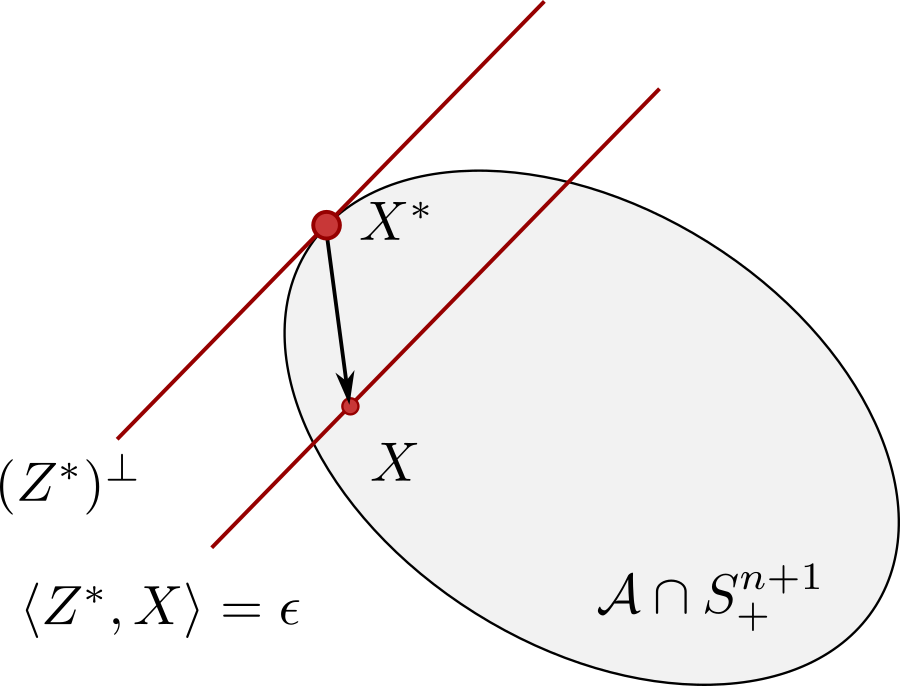
\includegraphics[width=0.5\textwidth]{images/feasibleset.png}
\end{center}
\caption{The feasible set of the Lovász SDP \ref{eqn:lovaszsdp} is a bounded convex set. It is given by the intersection of the set of positive semi-definite matrices $S_{+}^{n+1}$ and the affine space $\mathcal{A}$, as defined in the the text. $Z^{*}$ is the optimal solution of the SDP that is dual to \ref{eqn:lovaszsdp}. The primal optimal solution of \ref{eqn:lovaszsdp} is the unique point of intersection of the feasible set $\mathcal{A}\cap S_{+}^{n+1}$ and the subspace $(Z^{*})^{\perp}$ \cite{Bharti2019}. As such, the subspace $(Z^{*})^{\perp}$ is a supporting hyperplane of the feasible set, which lies entirely on one side of this hyperplane.  Furthermore, the set of $\epsilon$-suboptimal, feasible matrices is given by the intersection of $\mathcal{A}\cap S_{+}^{n+1}$ and $\{X\in \operatorname{Herm}(\mathbb{C}^{n+1})\,\vert\, \langle Z^{*}, X\rangle = \epsilon\}$ \cite{Bharti2019}.}
\label{fig:feasibleset}
\end{figure}

\begin{figure}
\begin{center}
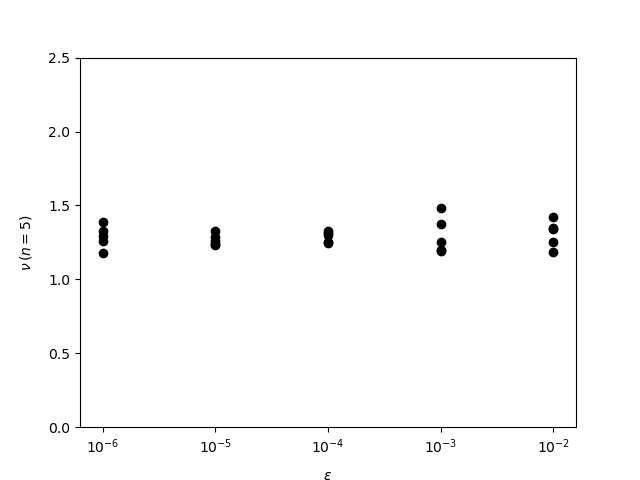
\includegraphics[width=0.7\textwidth]{images/propconst.png}
\end{center}
\caption{Numerical analysis of the proportionality constant $\nu(n)$ in Lemma \ref{lem:epssuboptgram}, for $n=5$. These values are computed by randomly generating $\sim 10^4$ feasible, $\epsilon$-suboptimal matrices, where $\epsilon$ ranges over several orders of magnitude. Plotted is the maximal ratio between deviation in Frobenius norm and suboptimality, $\nu_{\epsilon}(n=5)$, for $5$ independent trials. Each black dot corresponds to $\sim 10^4$ feasible, $\epsilon$-suboptimal matrices. We estimate the constant of proportionality to be $\max_{\epsilon} \nu_{\epsilon}(n=5)\sim 1.5$.}
\label{fig:propconst}
\end{figure}

\section{Assumptions}
\label{sec:kscontass}
The following is an as comprehensive as possible list of explicit or implicit assumptions that are required to self-test the reference quantum experiment \ref{eqn:ncycleideal}, on the basis of Theorem \ref{thm:contselftesting}:
\begin{enumerate}
    \item i.i.d.\ rounds $x,y \thinspace\vert\thinspace i,i\oplus 1$
    \item uncorrelated preparation and measurement devices,\\ freely random choice of measurement context $i,i\oplus 1$
    \item sharp (outcome-repeatable and minimally disturbing) measurements 
    \item cyclic compatibility
    \item to certify quantumness:
    \begin{enumerate}
    \item sequential measurements
    \begin{itemize}
        \item system not disturbed between measurements
    \end{itemize}
    \item information carrying capacity of the unknown system does not exceed ``simulable" bound (each measurement device is used only once) - memory assumption \cite{Bharti2019}
    
     \end{enumerate}
\end{enumerate}

Let us go through Assumptions 1-5 in order:

Assumptions 1, namely that the devices behave in the same way for every input-output round of the correlation experiment, is made in a large majority of current self-testing works \cite{Supic2020}. It allows us to lift relative frequencies observed in a correlation experiment to well-defined probability distributions $p(x,y\thinspace\vert\thinspace i, i\oplus 1)$ that are valid for all rounds of the protocol, a round being characterized by one input-output cycle for a given measurement context.

For a second, assume that Assumption 2 is not true, and consider the preparation and  measurement devices to be correlated. We express this in terms of some shared classical randomness $\lambda$. As noted in \cite{Miklin2020}, such shared randomness can render the task of self-testing futile. Consider a quantum experiment where, based on the value of $\lambda$, a device prepares $\rho_\lambda=U_\lambda \rho \thinspace U_\lambda^{\dag}$, with $U_\lambda$ unitary, and the measurement event $0,1 \,\vert\, i, i\oplus 1$ is characterized by a positive semi-definite operator $F_\lambda^{i,i\oplus 1}=U_\lambda F^{i,i\oplus 1} U_\lambda^{\dag}$. The probability $p(0,1 \thinspace \vert \thinspace i,i\oplus 1)=\int_{\Lambda} d\lambda\thinspace\mu(\lambda)\operatorname{tr}(\rho_\lambda F_\lambda^{i,i\oplus 1})=\operatorname{tr}(\rho F^{i,i\oplus 1})$. This correlation experiment with shared randomness is therefore operationally indistinguishable from one without, and we cannot hope to relate the physical experiment to the reference experiment via a single unitary operator, based on observed correlations alone.

The necessity of Assumption 3 for the soundness of the self-testing protocol was already highlighted in Sections \ref{sec:cswunsharp} and \ref{sec:complicationscont}. For unsharp quantum measurements, the class of odd $n$-cycle inequalities can be super-maximally violated by trivial POVM. Therefore, the CSW hierarchy falls apart and the Lovász SDP no longer characterizes optimal quantum violations of KS non-contextuality inequalities. Assumption 3 was critical in the above approach. Nevertheless, we would like to relax it - in a realistic setting, measurements will never be truly projective.

Assumption 4 is required by the CSW framework. If the measurements $i,i\oplus 1$ were not compatible, the measurement events in Figure \ref{fig:kcbsexclusivity} could not be related to well-defined projectors $\Pi_i$, even for sequential measurements, as the product of two non-commuting projectors is not necessarily a projector.

As Assumption 5 is extensive, we devote an entire section to it. We assume sequential measurements, as they allow us to bound classical simulations reproducing the statistics in a non-trivial manner, something we will examine in Section \ref{sec:memoryass}. We assume that the system is not disturbed in between sequential measurements, so that the measurement sequence $i,i\oplus 1$ corresponds to a well-defined projector like before.

\section{Sequential measurements and the memory assumption}
\label{sec:memoryass}
As described in Section \ref{sec:self-testing}, self-testing allows us to make powerful inferences about the quantum properties of a system. For applications of self-testing, the prime example being quantum key distribution (QKD), it is of great importance that the certificate not only encompasses the quantum state and measurements consistent with the maximal violation, but that the optimal input-output correlations also bear witness to the quantumness of the system. This means that we must exclude the possibility of the correlations being simulated by some classical mechanism, as this would for instance allow the copying of information and render the protocol information-theoretically insecure. To do so, we wish to study the resources a classical device requires, in order to simulate the ideal reference quantum realization. The odd $n$-cycle contextuality scenarios will be of particular interest to us. 
In the case of Bell inequalities, the relevant resources have been identified and studied extensively \cite{Brassard1999,Toner2003}. As highlighted in Section \ref{sec:bell}, assuming local causality and freely chosen detector settings, correlations that violate a Bell inequality are incompatible with a local hidden variable model description. Thus, classically simulating correlations that exhibit Bell non-locality requires superluminal communication (``communication cost") \cite{Toner2003} and would violate special relativity. For self-testing via Bell inequalities this means that, assuming any adversary is bounded by the no-signalling principle, the violation of a Bell inequality certifies quantumness, provided that both subsystems are indeed space-like separated. Analogously to Bell non-locality and the no-signalling principle, we wish to identify a physical principle that enables us to differentiate between a quantum system exhibiting KS non-contextuality and a classical mechanism simulating correlations that violate a KS non-contextuality inequality.
One strength of contextuality as a competing notion of nonclassicality is that contextuality experiments comprise a much broader class of experiments. In particular, generic contextuality experiments don't presuppose multiple space-like separated systems, but can consist of sequences of state preparations and measurements of a single system. However, this generality also complicates the analysis of the relevant resources required for simulating KS contextuality. Moreover, we can in principle never distinguish between a single-system quantum experiment exhibiting some input-output correlations and a classical pre-programmed computer simulating these \cite{Supic2020}. For Bell-type scenarios this possibility is circumvented by extending the experiment to multiple space-like separated subsystems. In Section \ref{sec:memoryass} we examine the ``memory cost" of KS contextuality \cite{Cabello2018,Kleinmann2011}: As we will see, the minimal internal entropy of a classical system emulating KS contextuality in many cases exceeds the information-carrying capacity of the quantum system it aims to emulate. To weed out the possibility of a classical mechanism producing the correlations, in \cite{Bharti2019} it is assumed that ``[$\dots$] the measured system has no more memory than its information carrying capacity".
However, for self-testing scenarios the information carrying capacity of the physical device is unknown.
One therefore has to justify imposing an upper bound on the unknown device's information carrying capacity to conclude quantumness. As we will see, these upper bounds have to be of the order of a few bits, which means that the required memory assumption is a very strong one indeed. 

In Section \ref{sec:protocols}, where we propose a self-testing protocol based on Spekkens contextuality, the cyclic compatibility and measurement sharpness assumptions will be replaced by assumptions about (approximate) operational equivalences of certain experimental procedures. The protocol will also assume an upper bound on the information carrying capacity of the unknown system. We will discuss its features in Section \ref{sec:discussion}.

Alternatively, Cabello proposes using Landauer's principle \cite{Cabello2018} to translate the memory cost of KS contextuality into a ``thermodynamical cost" \cite{Wiesner2012,Cabello2016}, in terms of heat the system dissipates when measured. We briefly sketch the general idea, however, as the minimal unit of Landauer heat a classical simulation must dissipate per measurement will be of the order $\sim k_BT$, this proposal is hardly viable in a realistic experimental setting:
For sufficiently long measurement sequences, a classical simulation with finite memory must ``forget" information about the past input-output sequence. It is as such a logically irreversible computation \cite{Wiesner2012}.
Landauer's principle states that whenever classical information is processed in a logically irreversible manner, for example when erasing a classical bit of information, the entropy of the environment increases by a corresponding amount. For the erasure (setting to zero) of a classical bit this entropy increase is at least $\Delta S_{env}\geq -\Delta S_{sys} = -(0-k_B\log(2))=k_B\log(2)$. This entropy increase is related to the heat dissipated to the environment reservoir via $\Delta Q= (\Delta S)\thinspace T$, meaning that the minimal amount of dissipated heat for the erasure of a single classical bit is given by $\Delta Q = k_B T \log(2)$.

\subsection{Setting and preliminary considerations}
We consider correlations experiments that consist of a series of sequential measurements for different measurement contexts $i,i\oplus 1$. Within quantum theory it does not matter whether we consider joint or sequential measurements of compatible observables, as both produce identical correlations. To that effect we will assume that our system is not perturbed between successive measurements. If one measurement is performed at time $t$ and another at $t' > t$, then we want the system's state to remain unchanged in the time interval $(t, t')$.

Let us now examine how, in an adversarial setting where correlations may not capture the outcome statistics of compatible and ideal quantum measurements, a classical device with an internal memory can simulate the input-output process characterized by the correlation experiment.

\subsection{Input-output processes as information transducers}
In most general terms, a KS contextuality experiment is an input-output process. To verify that an experiment producing a maximal violation of say the KCBS KS non-contextuality inequality is compatible with the ideal reference experiment, we may in principle perform an infinite sequence of measurements  $\oset{\leftrightarrow}{X}=\{\dots,\thinspace X_{-1},\thinspace X_{0},\thinspace X_{1},\thinspace\dots\}$, yielding an infinite sequence of outputs $\oset{\leftrightarrow}{Y}=\{\dots,\thinspace Y_{-1},\thinspace Y_{0},\thinspace Y_{1},\thinspace \dots\}$ \cite{Cabello2018}. Here, $\oset{\leftrightarrow}{X}$ and $\oset{\leftrightarrow}{Y}$ are bi-infinite sequences of random variables and define stochastic processes. The random variable $X_{i}$ represents the freely chosen random measurement at time $t=i\in\mathbb{Z}$, whereas the random variable $Y_{i}$ represents the output obtained when performing the measurement $X_{i}$ at time $i$. We assume that all $X_i$ and $Y_i$ take values from finite alphabets $\mathcal{X}$ and $\mathcal{Y}$; most of the measurements we will consider are dichotomic, i.e.\ $\vert\mathcal{Y}\vert=2$, as is the case for the KCBS KS contextuality scenario. Furthermore, we can distinguish the present $t=0$ and partition the processes $\oset{\leftrightarrow}{X}$, $\oset{\leftrightarrow}{Y}$ into past and future: $\oset{\leftarrow}{X}\thinspace\coloneqq \dots,\thinspace X_{t-2},\thinspace X_{t-1}$, $\oset{\rightarrow}{X}\thinspace\coloneqq X_t,\thinspace X_{t+1},\thinspace \dots$. The reference time is in fact arbitrary, as the stochastic processes we will consider turn out to be stationary. Any classical input-output mechanism producing a maximal violation that we cannot ``unmask" on the basis of correlations alone, must be consistent with the ideal reference input-output process.

Any classical apparatus simulating the reference correlations has the form of a general information transducer, transforming an input stochastic process into an output stochastic process \cite{Cabello2018}. A classical simulation is at all times $i$ in some well-defined internal state $S_i$ that holds information about the past input-output sequence $\oset{\leftarrow}{Z}\thinspace\coloneqq(\oset{\leftarrow}{X},\oset{\leftarrow}{Y})$, stored inside a memory. As the future process may be correlated with the past, the internal memory of the device allows it to produce statistically correct predictions. If we pass a valid input symbol from $\mathcal{X}$ (think of $\mathcal{X}$ as the $n$ measurement settings a verifier can choose from for the odd $n$-cycle scenario) to the transducer it will generate an output symbol in $\mathcal{Y}$, based on the information about the past encoded in the internal state prior to the input. We assume that the choice of measurement setting is freely random and not correlated with the internal state of the machine. The output may be accompanied by an update of the transducer's internal memory. One can think of this input-output process as feeding the transducer an infinite tape, whereby each tape cell contains a valid input symbol (choice of measurement). The transducer then generates an output, overwrites the corresponding tape cell with said output, and updates its internal state, see Figure \ref{fig:transducer}. Note that we will only consider the RAM memory cost of such a simulation, which relates to the number of memory bits the device needs to store the relevant historical information about the past process\footnote{alternatively, the RAM memory cost can be regarded as the uncertainty (in bits) in the internal state of the transducer.}, and in particular not to the memory required to store say output and transition probabilities.

\begin{figure}
    \centering
    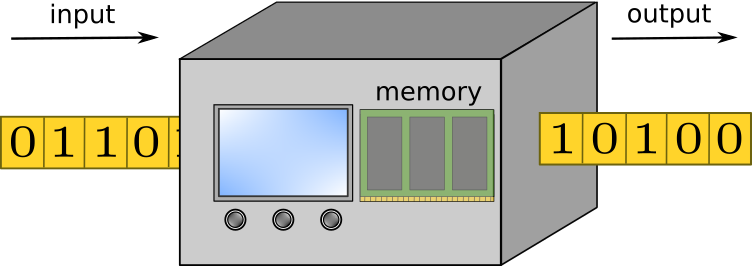
\includegraphics[width=0.6\textwidth]{images/transducer.png}
    \caption{A classical device simulating the ideal reference statistics of some KS-type experiment, consisting of sequential measurements. The device is fed a sequence of inputs (measurement choices) and produces outputs (measurement outcomes), based on its internal state prior to an input. The internal state of the device, which one can equate with a memory, stores relevant historical information about the past input-output process, on the basis of which the device generates the correct input-output statistics. After one input-output cycle, the device can update its memory state.}
    \label{fig:transducer}
\end{figure}

\begin{definition}[\cite{Barnett2015}]
An \emph{information transducer} is a tuple $(\mathcal{X},\mathcal{Y},\mathcal{S},\mathcal{T})$ where
\begin{itemize}
    \item $\mathcal{X}$, $\mathcal{Y}$ are the transducer's (finite) input and output alphabets,
    \item $\mathcal{S}$ is a (finite or countably infinite) set of internal memory states, and
    \item $\mathcal{T}\equiv\{p(S_{i+1}=s', Y_i=y\vert S_i = s, X_i=x)\}_{x,\thinspace y,\thinspace s,\thinspace s'}$ is the set of conditional ouput-transition probabilities.
\end{itemize}
More concretely, $p(S_{i+1}=s', Y_i=y\vert S_i = s, X_i=x)$ denotes the probability of the transducer outputting $y$ and transitioning to the internal state $s'$ after the $ith$ input-output cycle, conditioned on the input $x$ and internal state $s$.
\end{definition}

We require a valid classical model to produce statistics that are consistent with the infinite family of stochastic processes describing the quantum probabilities of the ideal reference experiment: $\{P(\oset{\leftrightarrow}{Y}|\oset{\leftrightarrow}{x})\}_{\oset{\leftrightarrow}{x}}$\thinspace, $\oset{\leftrightarrow}{x}$ being an instantiation of the input sequence $\oset{\leftrightarrow}{X}$.

Input-output transducers have been extensively studied within the field of computational mechanics. Of interest to us are memory-optimal classical models that produce the correct statistics $\{P(\oset{\leftrightarrow}{Y}|\oset{\leftrightarrow}{x})\}_{\oset{\leftrightarrow}{x}}$\thinspace. A transducer is memory-optimal if it stores the minimal amount of information about the past (in terms of number of bits) to make statistically correct future predictions. It has been shown that for stationary input-output processes there exists a unique memory-optimal transducer producing the correct statistics: the process' $\epsilon$-transducer \cite{Barnett2015}. The memory-optimal transducer does not store all information about the past $\oset{\leftarrow}{Z}$, as this may be highly redundant. In particular, the memory-optimal transducer does not differentiate between pasts that predict statistically identical futures. As such, the internal states of an $\epsilon$-transducer are given by the causal states of the process. 

\begin{definition}
Let $\oset{\leftarrow}{X}$, $\oset{\rightarrow}{X}$ denote the past and future stochastic input processes, respectively.
The \emph{causal states} $[\oset{\leftarrow}{z}]$ of an input-output process $\oset{\leftrightarrow}{Y}|\oset{\leftrightarrow}{X}$ are the equivalence classes on the set of pasts $\oset{\leftarrow}{z}$ with respect to the equivalence relation
\begin{equation*}
\oset{\leftarrow}{z}\;\sim_\epsilon\;\oset{\leftarrow}{z}'\;\mathrel{\vcentcolon\Leftrightarrow} \;P(\oset{\rightarrow}{Y}|\oset{\rightarrow}{X},\oset{\leftarrow}{Z}=\oset{\leftarrow}{z})= P(\oset{\rightarrow}{Y}|\oset{\rightarrow}{X},\oset{\leftarrow}{Z}=\oset{\leftarrow}{z}').
\end{equation*}
\end{definition}

\subsection{Memory-optimal classical simulation of quantum correlations}
In \cite{Cabello2018} it is shown that, for a ``causally complete" KS contextuality reference experiment, the causal states of the process' $\epsilon$-transducer correspond one-to-one to the possible quantum states $\{\ket{\Phi_{\oset{\leftarrow}{z}}}\}_{\oset{\leftarrow}{z}}$ the system can occupy after all past measurements $\oset{\leftarrow}{x}$. The assumption of causal completeness holds for many KS contextuality scenarios and in the following we will examine the odd $n$-cycle KS contextuality scenarios, in particular the KCBS scenario for $\text{n}=5$. In \cite{Cabello2018}, the same analysis is performed for the Peres-Mermin (see Section \ref{sec:4dim}) and Yu-Oh (see Section \ref{sec:kcbs}) sets of measurements.

For all ideal odd $n$-cycle reference experiments, the number of possible post-measurement states tends to infinity when we increase the number of measurements in our sequence. However, the post-measurement states are not all equally probable. Figure \ref{fig:causalstates} illustrates this behaviour for the KCBS scenario $\text{n}=5$.

\begin{figure}
        %\centering
        \begin{subfigure}{0.5\textwidth}
            \centering
            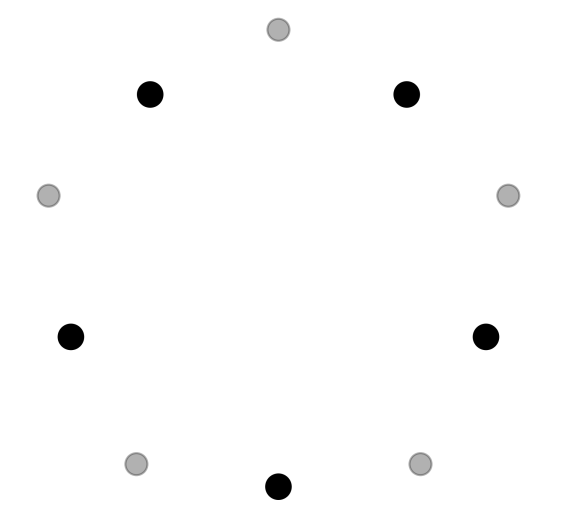
\includegraphics[width=0.7\textwidth]{images/n=5,mnts=1.png}
            \caption{one measurement}
        \end{subfigure}
        \hfill
        \begin{subfigure}{0.5\textwidth}
            \centering 
            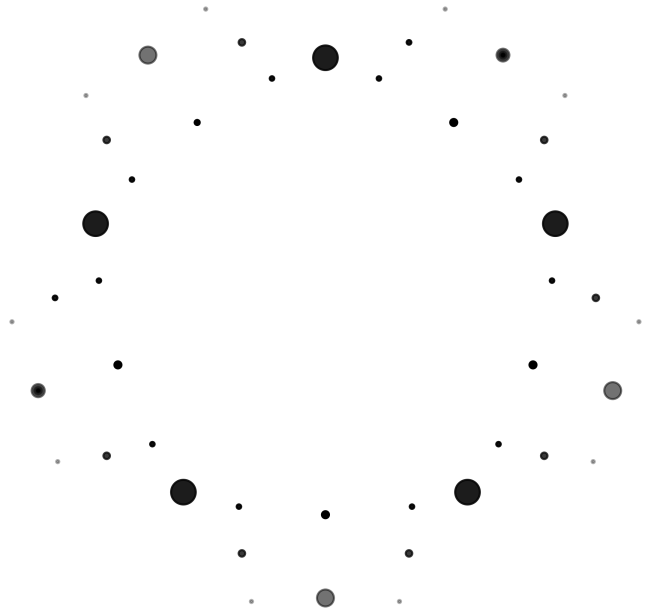
\includegraphics[width=0.7\textwidth]{images/n=5,mnts=3.png}
            \caption{three measurements}
        \end{subfigure}
        \vskip\baselineskip
        \begin{subfigure}{0.5\textwidth}
            \centering 
            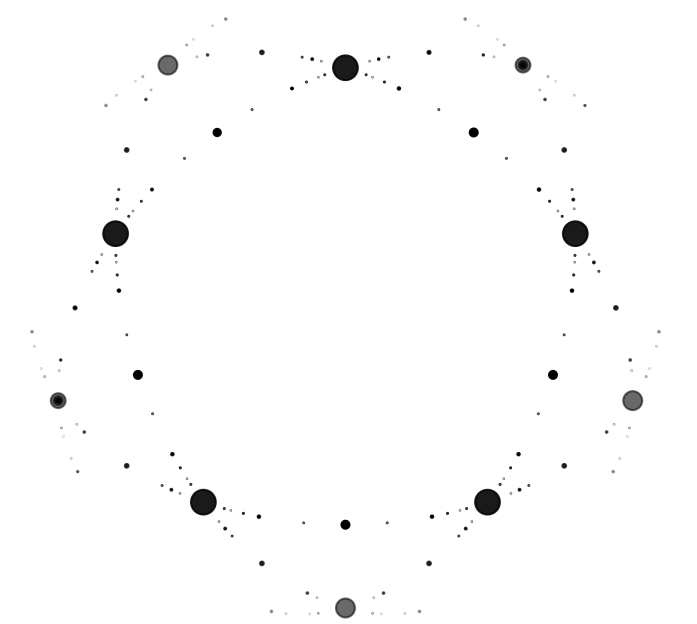
\includegraphics[width=0.7\textwidth]{images/n=5,mnts=5.png}
            \caption{five measurements}
        \end{subfigure}
        \hfill
        \begin{subfigure}{0.5\textwidth}
            \centering 
            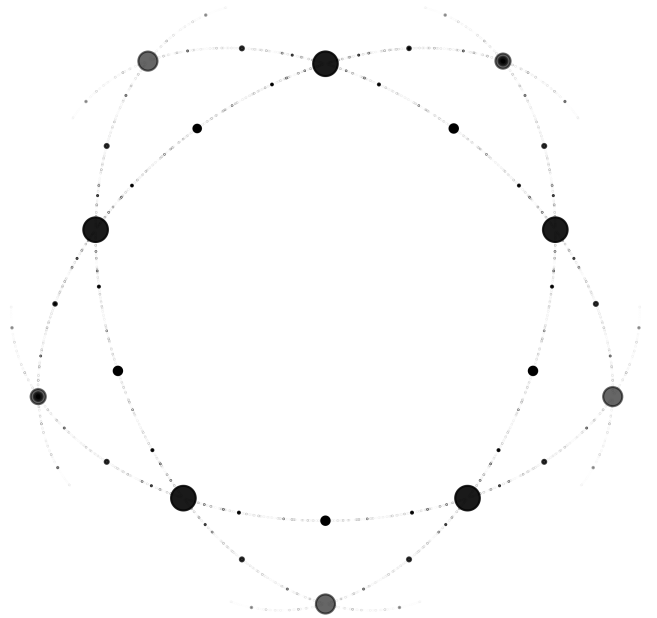
\includegraphics[width=0.7\textwidth]{images/n=5,mnts=10.png}
            \caption{ten measurements}
        \end{subfigure}
        \caption{Possible post-measurement quantum states after one, three, five, and ten measurements for the ideal KCBS experiment. The components of the post-measurement quantum states w.r.t.\ the standard qutrit basis are all real. The phases (signs) of the real qutrit states are chosen such that the corresponding vectors lie on a joint semisphere of $\mathbb{R}^3$. What is plotted are centered views of the three-dimensional plots along the negative x direction. As can be seen, the number of possible post-measurement states increases with the number of sequential measurements. The volume of a scattered point is proportional to the probability of the system being in that state after the measurements. The probability distribution over possible post-measurement quantum states becomes approximately stationary for large measurement sequences. The fact that all states lie on one of five semi-circles is a consequence of the compatibility structure of the five KCBS measurements. Analogous plots are obtained in \cite{Cabello2018} for the Peres Mermin and Yu-Oh KS contextuality scenarios.}
        \label{fig:causalstates}
    \end{figure}

Problematically, the process describing the ideal quantum experiment is not stationary, i.e.\ not invariant under translations in time, as can be seen from Figure \ref{fig:causalstates}. However, if we ``truncate" the process and consider only input-output cycles after sufficiently many initial measurements, the probability distribution over quantum states and by extension the stochastic process describing the experiment becomes stationary for all practical purposes. We only have a notion of the memory-optimal statistics-emulating classical model for the case of stationary processes. For this reason we will always consider the truncated input-output process.

To numerically compute the memory cost, we consider all possible measurement sequences of a given length k. The statistical complexity of the process (RAM memory cost) is then the Shannon entropy $H=-\sum_ip_i\log_2p_i$ of the probability distribution over all achievable post-measurement quantum states after $k$ measurements, in the limit of $k\rightarrow\infty$ \cite{Cabello2018,Barnett2015}. Recall that this probability distribution becomes approximately stationary, reflected by the above expression converging. We find the number of bits (RAM) needed by a memory-optimal simulation of the ideal reference KCBS experiment to be just over 4. The statistical complexity thus exceeds the information carrying capacity $\mathcal{C}=\log_2(3)$ of the reference qutrit. In \cite{Cabello2018}, the same qualitative behaviour is observed for the Peres-Mermin and Yu-Oh sets of measurements, both of which exhibit state-independent KS contextuality. 

An interesting feature we observe is that the memory cost of simulating the ideal reference experiment for odd $n$-cycle contextuality scenarios with $\text{n}\geq5$ odd increases with the cycle length $n$, as is shown in Figure \ref{fig:ncycleRAM}. However, this increase is only logarithmic. Furthermore, what does not change is the fact that, no matter the cycle length, we need to assume an upper bound on the unknown device's information carrying capacity, in order to conclude quantumness. Additionally, we need to assume that each measurement device is used only once, requiring a potentially infinite supply, as otherwise the measurement device, and not the system whose information carrying capacity we bound, could retain memory about the past stochastic process.

\begin{figure}
        \centering
        \begin{subfigure}{\textwidth}
            \centering
            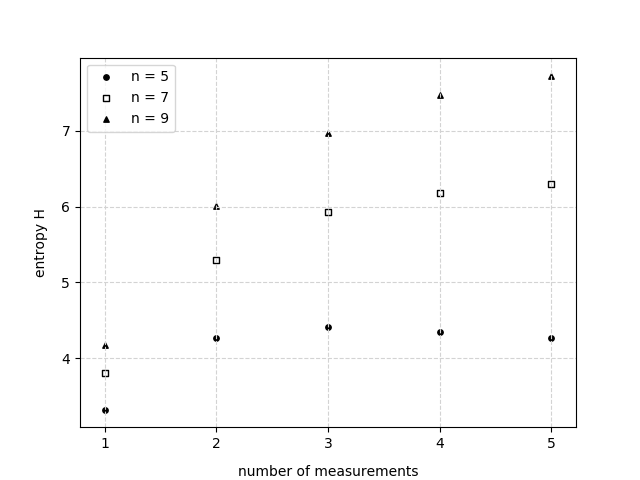
\includegraphics[width=0.7\textwidth]{images/allentropies.png}
            \caption{Plotted is the Shannon entropy of the probability distribution over all achievable post-measurement quantum states after a given number of measurements for the 5, 7, and 9-cycle KS contextuality scenarios. The probability distribution over possible post-measurement quantum states becomes approximately stationary for a sufficiently large number of measurements and the entropies thus saturate. This stationary limit of $H$ is the process' RAM memory cost, and it increases with an increasing cycle length}
        \end{subfigure}
        \vskip\baselineskip
        \begin{subfigure}{\textwidth}
            \centering 
            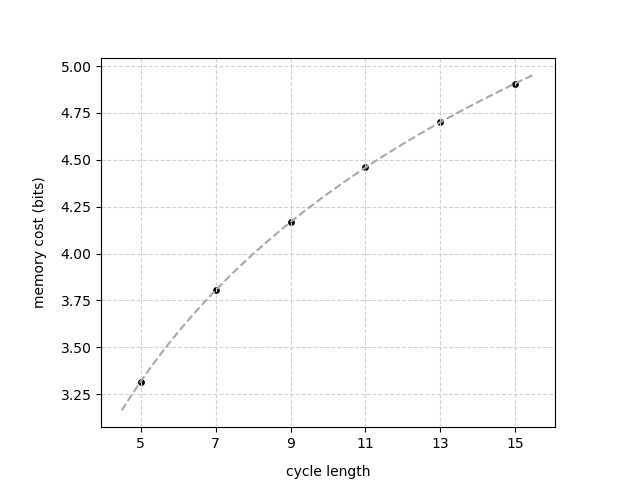
\includegraphics[width=0.7\textwidth]{images/memorycost.png}
            \caption{The RAM memory cost of classically simulating the ideal reference experiment for $n$-cycle KS contextuality scenarios increases logarithmically with the number of ideal measurements obeying cyclic compatibility that have to be implemented.}
        \end{subfigure}
        \caption{The RAM memory cost of classically simulating the ideal reference experiment for odd $n$-cycle KS contextuality scenarios in terms of the cycle length $n$.}
        \label{fig:ncycleRAM}
\end{figure}

Note that in Figure \ref{fig:ncycleRAM} only the asymptotic values of $H$ are physically relevant, characterizing the stationary regime. We have in fact adapted the protocol in \cite{Bharti2019}, by allowing the verifier to choose between $n$ measurements for every input. In particular, the verifier is not limited to just two sequential measurements within one context $i,i\oplus 1$, but can perform any measurement sequence in $\{1,\dots,n\}^m$, where $m$ is the length of the sequence. This comes with an increased measurement complexity, and the verifier must check for compatibility with the ideal reference experiment for $n^m$ measurement sequences, by comparing $n^m(2^m-1)$ correlations to the expected statistics. The measurement sequences have to be sufficiently long to approximate the stationary regime. In fact, for just two sequential measurements $i,i\oplus 1$, as proposed in \cite{Bharti2019}, one can find a classical model that reproduces the correlations of the ideal reference experiment, and requires less than one bit of memory. An information transducer with these properties is given in Figure \ref{fig:twomnts}. As such, the simulable bound on the information carrying capacity no longer exceeds the information carrying capacity of a qutrit. This highlights the need for an increased measurement complexity.

\begin{figure}
\centering
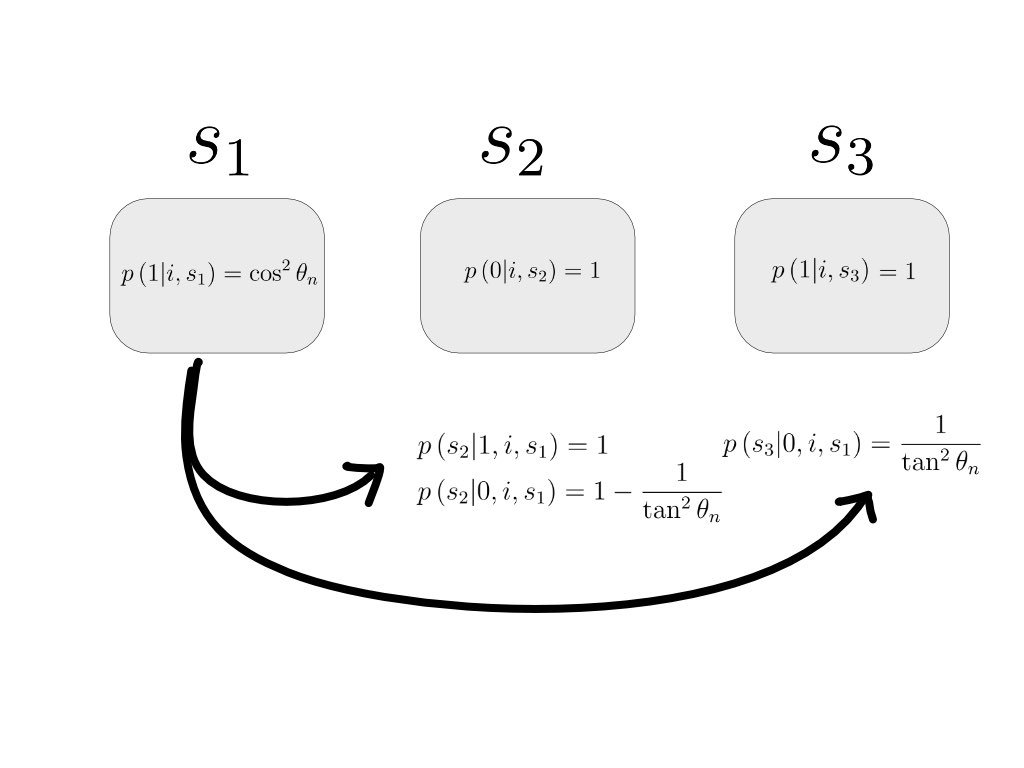
\includegraphics[width=0.8\textwidth]{images/twomnts.jpg}
\caption{Simple classical information transducer with three internal memory states, $s_1, s_2, s_3$, which reproduces all correlations of the ideal odd $n$-cycle experiment, provided that the experimenter performs only two sequential measurements $i, i\oplus 1$. The rectangles with grey border give the outcome probabilities, conditioned on the respective memory state $s_j$ and measurement $i$. The arrows indicate transitions in the internal state, and the respective conditional transition probabilities are given. Prior to each input-output cycle $i,i\oplus 1$, the transducer's memory is reset to the state $s_1$.
The memory cost of this simulation, i.e. the maximal uncertainty in the internal memory state of the machine, is less than one bit (after one measurement, the system is in one of two states with unequal probability), and in particular does not exceed the qutrit information carrying capacity. This simple example is meant to motivate an increased measurement complexity, in order to establish a clear separation in terms of resources between the ideal qutrit and any classical simulation.}
\label{fig:twomnts}
\end{figure}




